\chapter{Wykorzystane technologie}

Projekt został zrealizowany pod systemem Windows 10 oraz Mac OS X El Capitan. 

\section{C}
Z racji, iż sercem robota jest procesor z rodziny STM, wybór technologii został ograniczony do języka C lub C++. Wybrano język C z powodów optymalizacyjnych oraz małego stopnia skomplikowania programu. 


Oprogramowanie zostało stworzone w środowisku Eclipse z dodatkiem AC6 wspierającym platformę STM32.

\subsection{HAL}
HAL (Hardware Abstraction Layer) jest biblioteką będącą wysokopoziomowym interfejsem służącym do konfiguracji peryferiów mikrokontrolera. Zdecydowano się na wyżej wspomnianą bilbiotekę z powodu bardzo przejrzystej dokumentacji oraz łatwości użytkowania. Dodatkowo użyto środowiska CubeMX, które udostępnia graficzny interfejs, który pozwala na stosunkowo łatwą oraz intuicyjną konfigurację procesora oraz wygenerowanie projektu w języku C wraz z użyciem bibliotek HAL.


Na rysunku ~\ref{fig:cubemx} zilustrowano konfigurację peryferiów użytego procesora w środowisku CubeMX.   

\begin{figure}[H]
	\centering
		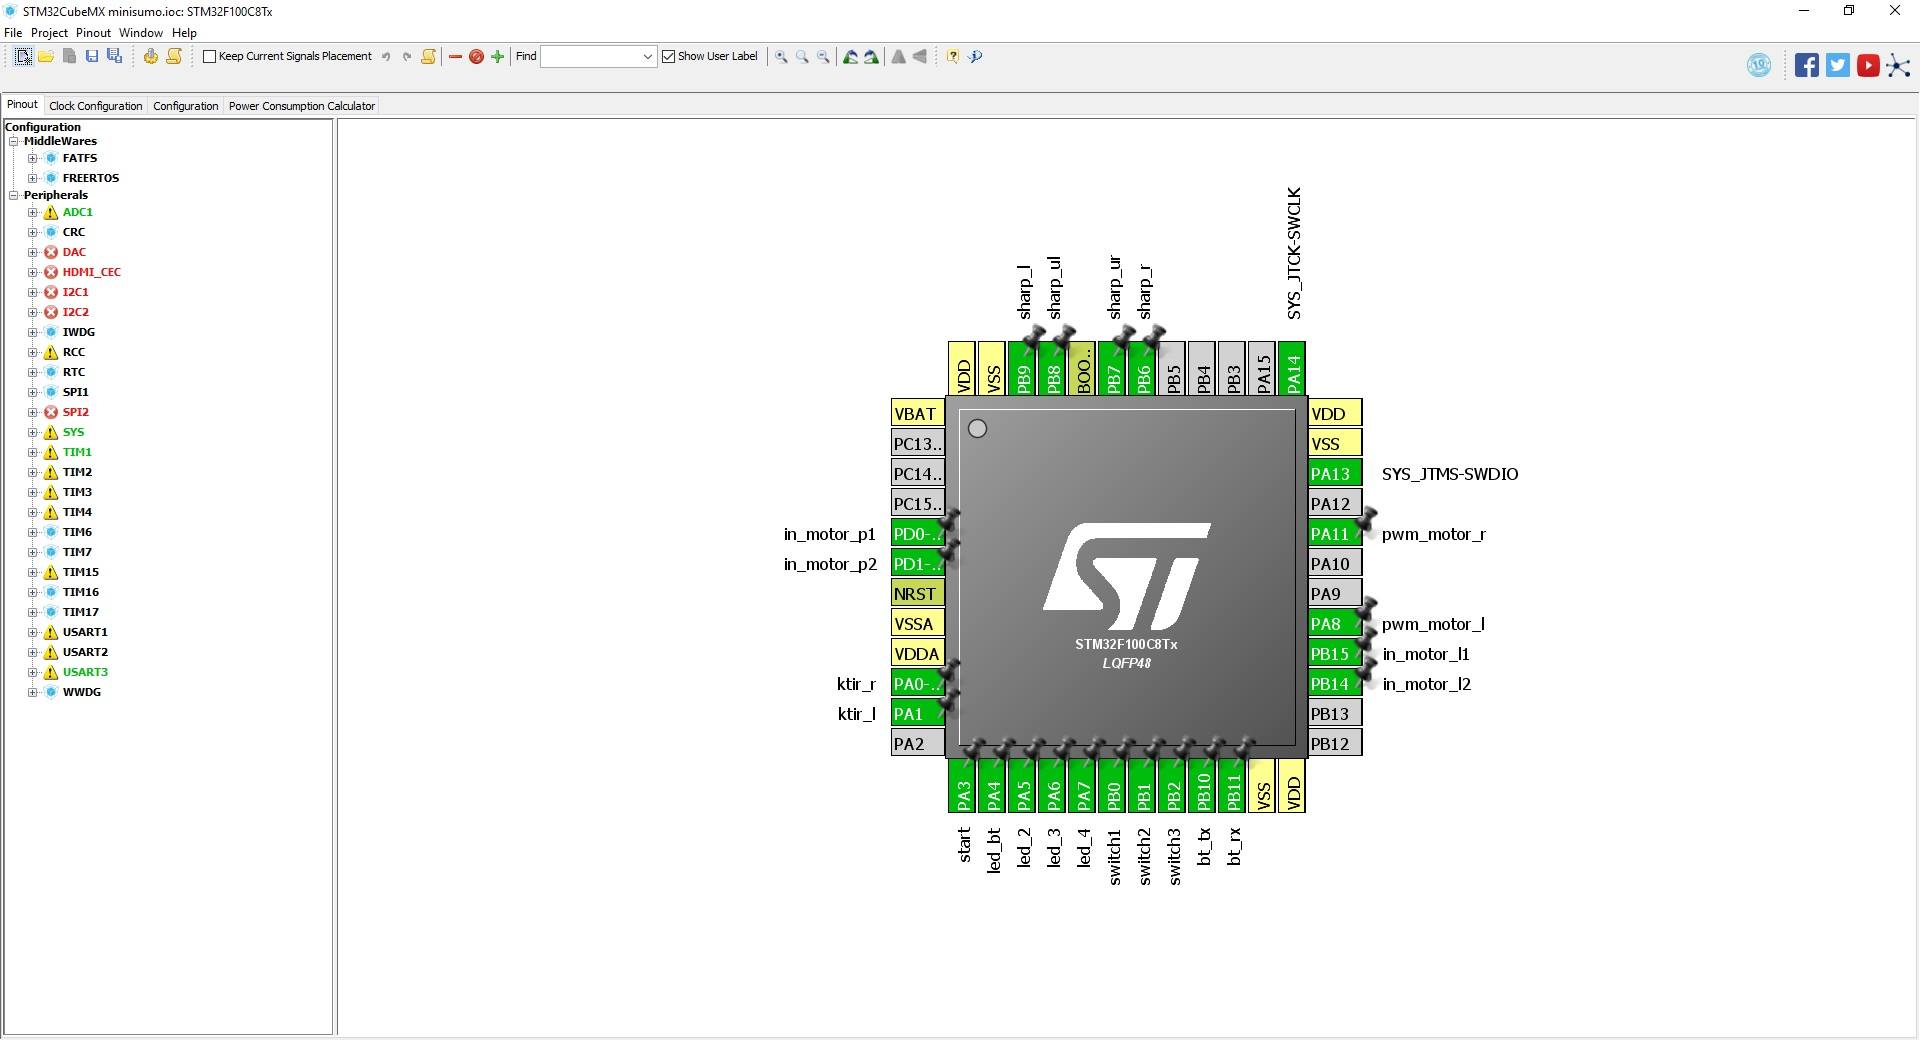
\includegraphics[width=0.75\linewidth]{pic02/cubemx.jpg}
	\caption{Konfiguracja peryferiów użytego procesora STM32F100C8T6B - LQFP48.}
	\label{fig:cubemx}	
\end{figure}

\section{Swift}
Swift jest językiem natywnym (następcą języka Objective-C) zaprezentowanym przez Apple Inc. w 2014 roku. Wykorzystywany jest do tworzenia oprogramowania na platformy macOS oraz iOS. W pracy dyplomowej użyto wersji języka 3.0, ponieważ była to najnowsza wersja wspierana przez docelowe urządzenie, którym był telefon iPhone 5.

Środowiskiem użytym do tworzenia aplikacji mobilnej w technologii Swift był Xcode, którego dużym atutem jest występowanie graficznego interfejsu umożliwiającego tworzenie widoków aplikacji. Dzięki temu tworzenie aplikacji jest bardziej intuicyjne oraz pozwala na sprawne wprowadzanie zmian w tworzonych widokach.

Na rysunku ~\ref{fig:xcode} zilustrowano środowisko Xcode wraz z widokami aplikacji oraz zależnościami między nimi.   

\begin{figure}[H]
	\centering
		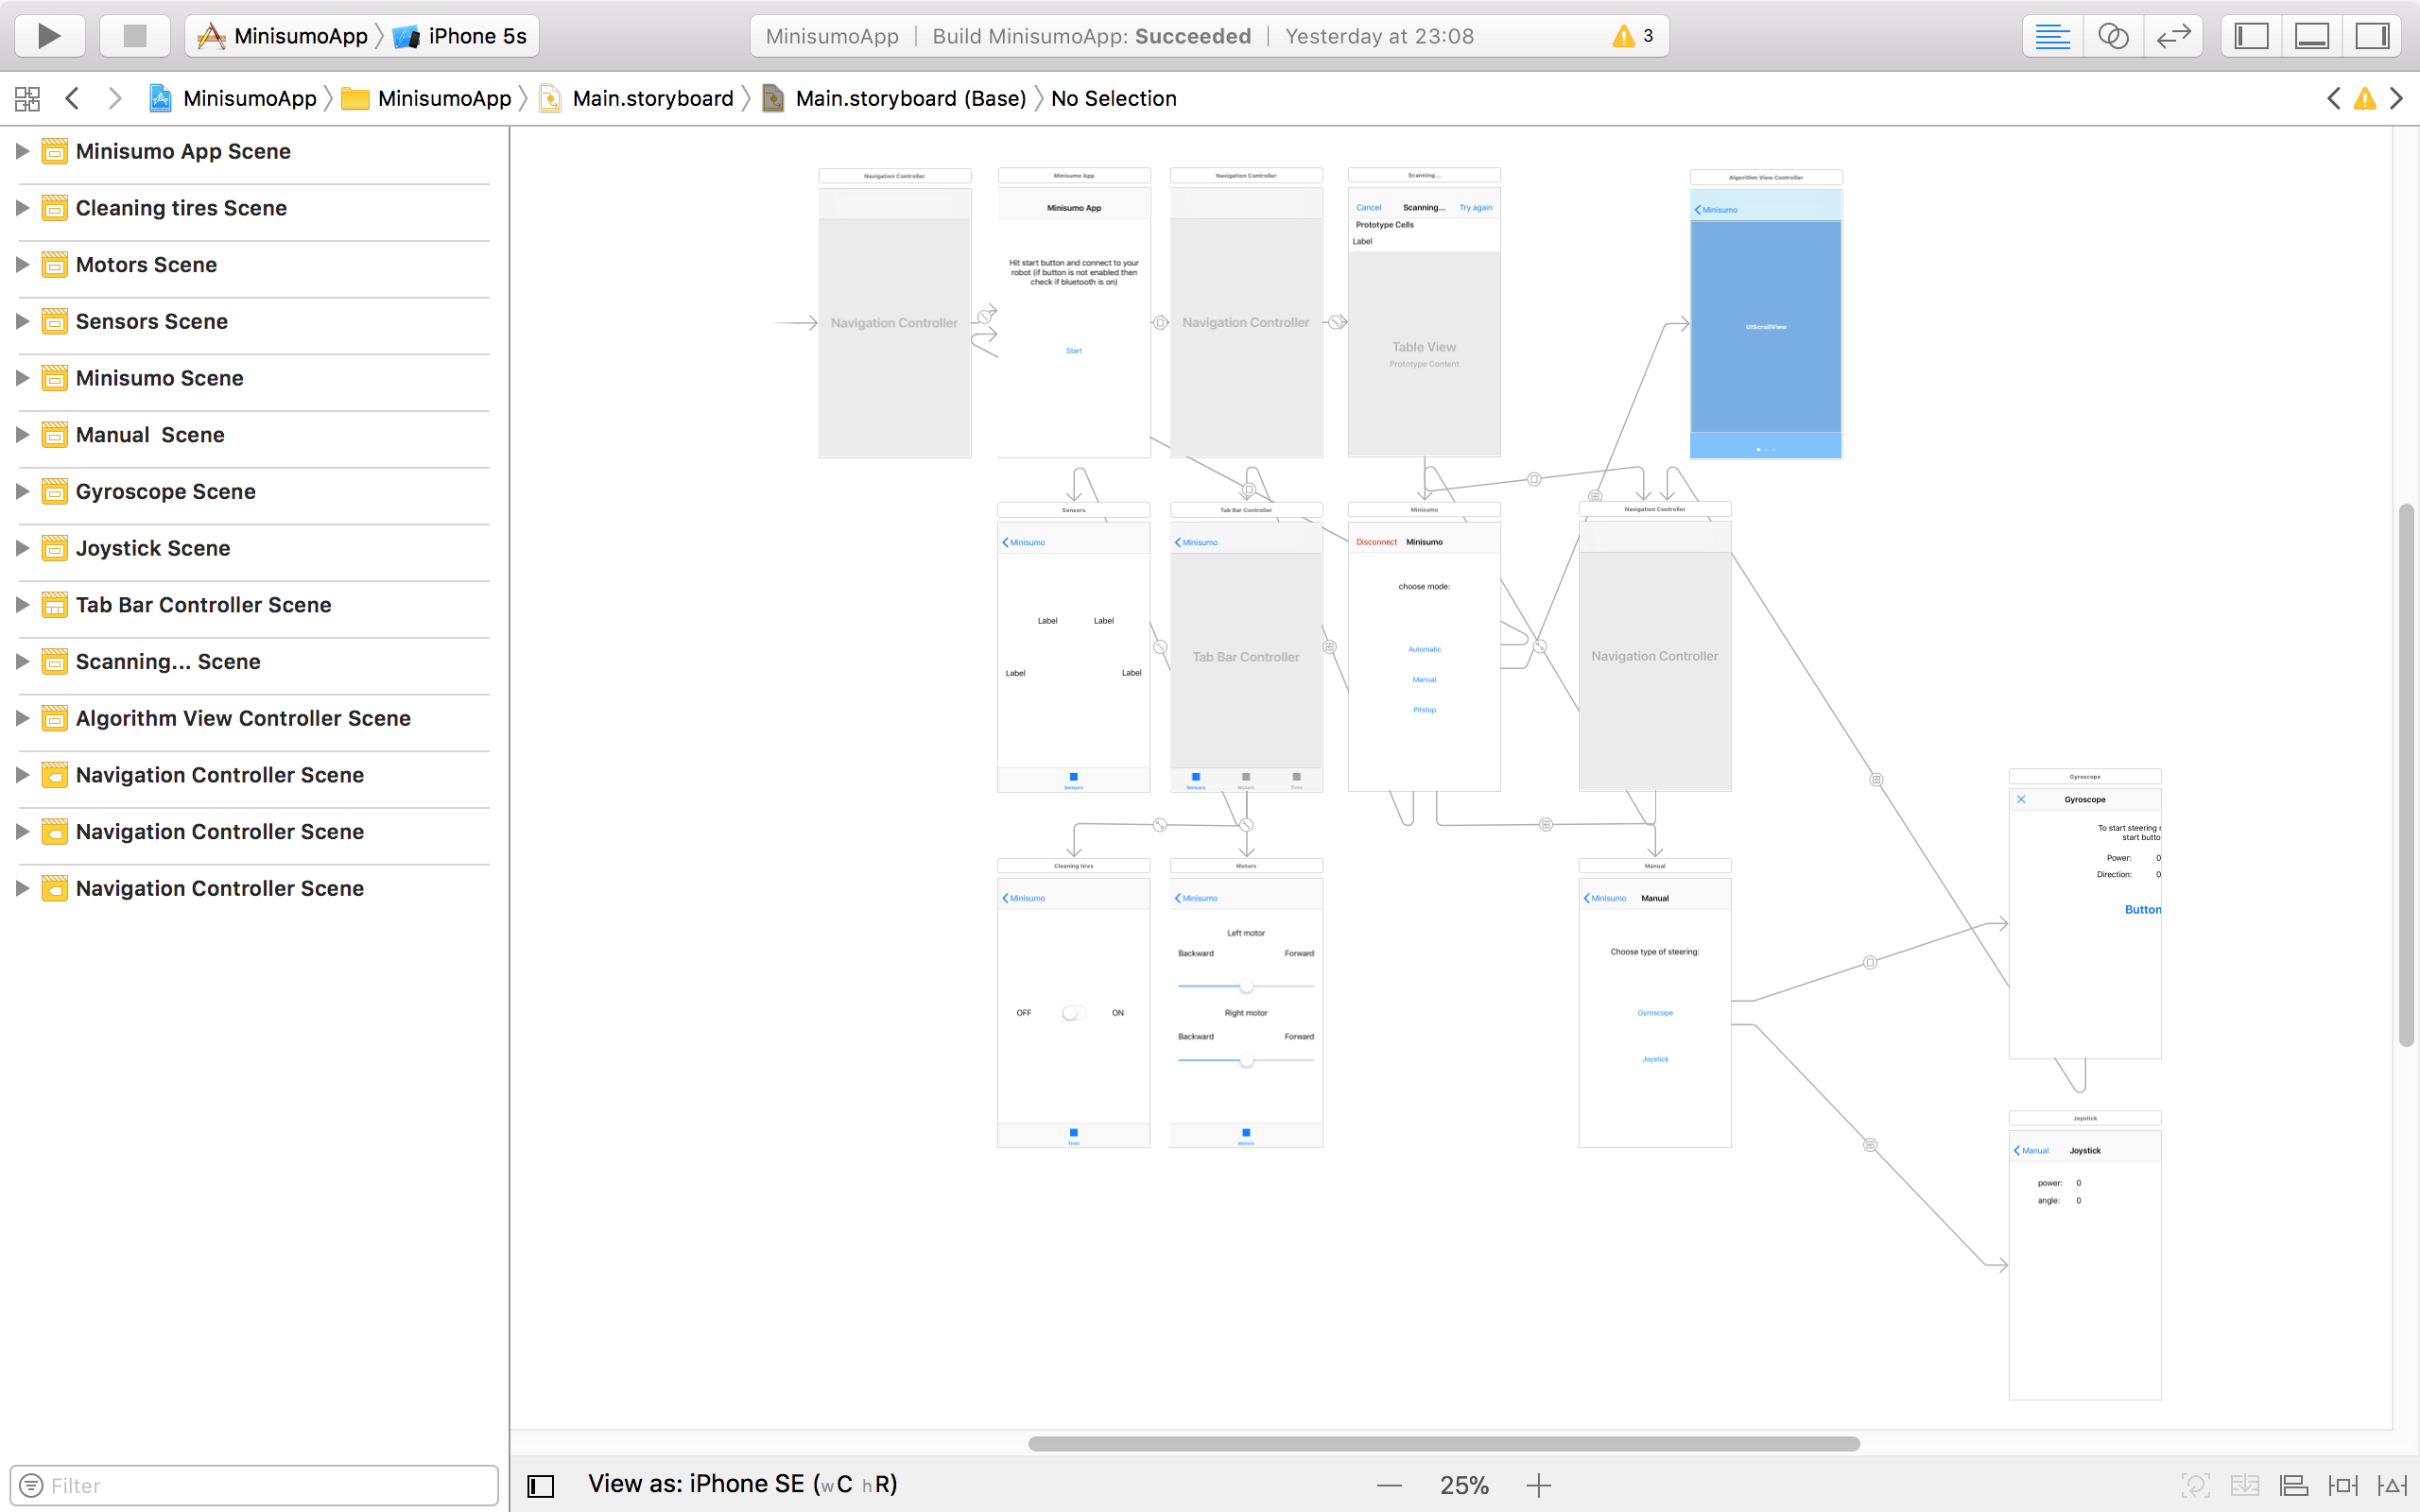
\includegraphics[width=0.75\linewidth]{pic02/xcode}
	\caption{Środowisko Xcode.}
	\label{fig:xcode}	
\end{figure}

\subsection{UIKit}
\subsection{CoreBluetooth}
\subsection{CoreGraphics}
\subsection{CoreMotions}

\section{Arduino}
